%
% Documento: Introdução
%

\chapter{Introdução}\label{chap:introducao}

Desde que a \textit{World Wide Web} foi proposta pelo cientista e pesquisador britânico Tim Bernes-Lee em 1989 \cite{WebHistory}, as páginas \textit{web} vêm mudando de maneira acelerada. Nos últimos 4 anos, o tamanho médio de uma página \textit{web} passou de 769kB para 2061kB, um expressivo aumento de 168\%, esse fato pode ser percebido observando os gráficos nas Figuras \ref{fig:httpcontenttype2011} e \ref{fig:httpcontenttype2015}, obtidas no \textit{website} HTTP Archive\footnote{http://httparchive.org/}.

O primeiro gráfico foi gerado com dados de 15 de Abril de 2011 e o segundo com dados de 15 de Abril de 2015 e os dois mostram a média de \textit{bytes} por página por tipo de conteúdo nas páginas \textit{web}. Mas a informação mais relevante está localizado na parte debaixo do gráfico e mostra o tamanho médio de uma página \textit{web} nas respectivas datas.

\begin{figure}[!htb]
    \centering
    \caption{Média de Bytes por Página por Tipo de Conteúdo em 2011}
    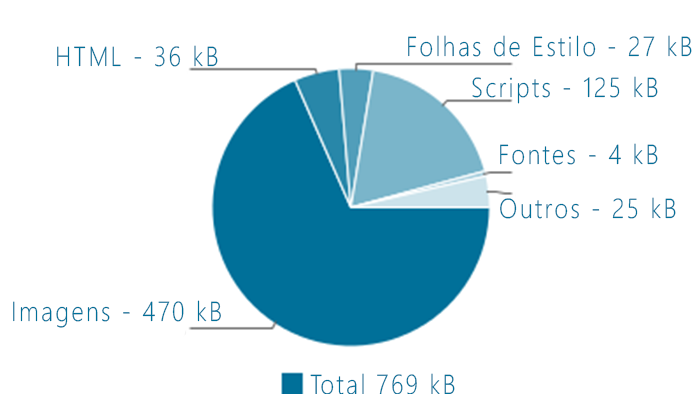
\includegraphics[width=0.6\textwidth]{./04-figuras/introducao/bytes_content_type_april_2011}
    \fonte{Adaptado de \citeonline{HttpArchiveContentType2011}}
    \label{fig:httpcontenttype2011}
\end{figure}

\begin{figure}[!htb]
    \centering
    \caption{Média de Bytes por Página por Tipo de Conteúdo em 2015}
    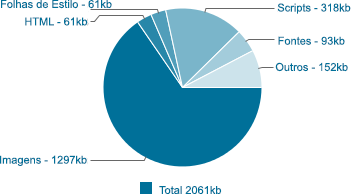
\includegraphics[width=0.6\textwidth]{./04-figuras/introducao/bytes_content_type_april_2015}
    \fonte{Adaptado de \citeonline{HttpArchiveContentType2015}}
    \label{fig:httpcontenttype2015}
\end{figure}

Apesar dessa grande mudança no tamanho das páginas (e consequentemente dos \textit{websites}), a maneira como \textit{websites} são entregues dos servidores para os clientes não sofreu nenhuma alteração desde 1999, ano de lançamento da RFC 2616 que especificou o HTTP/1.1 \cite{RFC2616}. Como explicado por \citeonline{Tanenbaum}, o HTTP é um protocolo simples na camada de aplicação de requisições e respostas que é executado em cima da camada de transporte do protocolo TCP. \citeonline{Tanenbaum} ainda diz que o HTTP ficou famoso por ser fácil de entender e implementar e ao mesmo tempo cumprir sua função de transferência de recursos em rede com um bom desempenho. Contudo, o aumento no tamanho dos \textit{websites} começou a fazer com que o tempo de resposta das páginas \textit{web} ficasse muito grande e, como mudanças no HTTP seriam muito difíceis, pois teriam de envolver esforços de muitas partes interessadas na \textit{World Wide Web} (como fabricantes de navegadores e mantenedores de servidores), os desenvolvedores passaram a ter de criar outras formas de resolver esse problema.

Técnicas de otimização de desempenho passaram a ser estudadas e implementadas por muitas empresas que queriam ter seus \textit{websites} entregues mais rapidamente a seus clientes. Por muitos anos, a grande maioria dessas empresas focou seus esforços em otimizações para o \textit{back-end}, principalmente para os seus servidores, o que hoje em dia pode ser considerado um erro. Como explicado por \citeonline[p.~5]{HighPerformance} no que ele chamou de "Regra de Ouro do Desempenho": "Apenas 10-20\% do tempo de resposta do usuário final são gastos baixando o documento HTML. Os outros 80-90\% são gastos baixando todos os componentes da página.".

Dessa forma fica claro que técnicas de otimização de desempenho para o \textit{front-end} dos \textit{websites} deveriam se tornar prioridade quando procura-se melhorar o tempo de resposta para o usuário final. Para entender o quão importante esse tempo de resposta se tornou para empresas que baseiam seus negócios em vendas de serviços ou produtos na Internet, basta observar os dados da tabela \autoref{tab:impactodesempenho} expostos por Steve Souders na conferência Google I/O de 2009:

\begin{table}[h]
	\centering
	\caption{Impacto do desempenho de \textit{website} na receita.\label{tab:impactodesempenho}}
	\begin{tabular}{lcl}
		\hline
			\textbf{Empresa} & \multicolumn{1}{l}{\textbf{Piora no tempo de resposta}} & \textbf{Consequência}  \\
		\hline
			Google Inc.      & +500ms                                                  & -20\% de tráfego       \\
			Yahoo Inc.       & +400ms                                                  & -5\% a -9\% de tráfego \\
			Amazon.com Inc.  & a cada +100ms                                           & -1\% de vendas         \\           
		\hline
	\end{tabular}
	\fonte{\cite{GoogleIO2009}}
\end{table}

Steve Souders tornou-se um grande evangelizador da área de otimização de desempenho de \textit{front-end} de \textit{websites}. Em seus livros, \textit{High Performance Websites} \cite{HighPerformance} e \textit{Even Faster Websites} \cite{EvenFaster}, o autor ensina técnicas de como tornar \textit{websites} mais rápidos, focando nos componentes das páginas. Em 2012, ele lançou seu terceiro livro, \textit{Web Performance Daybook} \cite{WebPerformance}, como um guia para desenvolvedores que trabalham com otimização de desempenho de \textit{websites}.

\section{Motivação}
\label{sec:motivacao}

Após mais de 15 anos sem mudanças, o protocolo HTTP receberá uma atualização. A nova versão do protocolo, chamada de HTTP/2, teve sua especificação aprovada no dia 11 de Fevereiro de 2015, \cite{HTTP2Spec}, e deverá começar a ser implantada, a partir de 2016. Muitas mudanças foram feitas com o objetivo de melhorar o desempenho e a segurança da \textit{Web}. Além disso, o HTTP/2 foi desenvolvido para ser compatível com suas versões anteriores, não sendo necessárias mudanças em servidores e aplicações antigas para funcionar no novo protocolo.

Com as novas funcionalidades do HTTP/2 a caminho, algumas coisas devem mudar na área de otimização de desempenho de \textit{websites}. Como pode ser percebido no trabalho de \citeonline{HTTP2Explained}, o HTTP/2 foi desenvolvido para melhorar o desempenho de todos os \textit{websites} e aplicações \textit{web}, e não apenas dos poucos que podem aplicar técnicas de otimização. Isso torna difícil uma previsão do resultado da aplicação de técnicas desenvolvidas para os protocolos HTTP/1.0 e HTTP/1.1. \citeonline{HighPerformanceBrowserNetworking} acredita que algumas das técnicas antigas podem não apenas não melhorar o desempenho dos \textit{websites} como podem acabar piorando o tempo de resposta para o usuário final.

No decorrer dos próximos anos o HTTP/2 deve seguir o mesmo caminho do HTTP/1.1 e se tornar o protocolo mais utilizado da \textit{Web}. Apesar de todo o esforço do HTTPbis (grupo responsável por desenvolver a especificação do HTTP/2) para desenvolver um protocolo que garanta o melhor desempenho de \textit{websites} e aplicações, sempre é possível ser mais rápido se as medidas certas forem tomadas. Sendo assim, as técnicas de otimização existentes devem ser analisadas quando aplicadas ao novo protocolo para saber como irão de comportar e o HTTP/2 deve ser estudado para saber se novas técnicas de otimização de desempenho serão necessárias.

\section{Objetivos}
\label{sec:objetivos}

Este trabalho tem como objetivo analisar o comportamento de técnicas de otimização de desempenho de \textit{websites} desenvolvidas por Steve Sourders para os protocolos HTTP/1.0 e HTTP/1.1 quando aplicadas a \textit{websites} usando o protocolo HTTP/2.

Para a realização do objetivo principal, os seguintes objetivos específicos foram determinados:

\begin{enumerate}
	\item Fazer uma análise comparativa das versões do protocolo HTTP
	\item Avaliar os ganhos de desempenho das técnicas propostas por Steve Souders ao aplicá-las ao HTTP/2
\end{enumerate}